\documentclass{article}
\usepackage{amsmath,amssymb,amsthm}
\usepackage{graphicx}
\usepackage[pdfborder= 0 0 0,citecolor=black,linkcolor=black,colorlinks=true,bookmarksopen=true]{hyperref}
\usepackage[notref]{showkeys}
\usepackage{caption}
\usepackage{subcaption}
\usepackage{algorithm}
\usepackage{algorithmicx}
\usepackage{algpseudocode}
\usepackage{tikz}
\usetikzlibrary{matrix}
\usepackage{tikz-3dplot}
\usepackage{pgfplots}
\usepackage{authblk}
\usepackage[pagewise]{lineno}
\usetikzlibrary{plotmarks}
\author[1,*]{P.A. Browne}
\affil[1]{Department of Meteorology, University of Reading, UK}
\affil[*]{Correspondence to p.browne@reading.ac.uk}
\title{THE TITLE}
\makeatletter \AtBeginDocument{ \hypersetup{pdftitle= {\@title},pdfauthor= {\@author}}} \makeatother

\date{\today}


\newcommand{\D}[2]{\frac{\partial #1}{\partial #2}}
\theoremstyle{plain}
\newtheorem{algo}{Algorithm}
\theoremstyle{definition}
\newtheorem{defn}{Definition}
\theoremstyle{theorem}
\newtheorem{theorem}{Theorem}
\begin{document}
\linenumbers
{\huge \today}

A naive approach to r-adaptivity on the sphere would be to map the surface onto the plane, use an established method to solve a mesh redistribution problem on the plane, then map back to the sphere. As shown in Figure \ref{commutative_diagram} the desired map $T$ could be written as a composition of mappings as $T = g^{-1} \circ t \circ g$.

\begin{figure}\begin{center}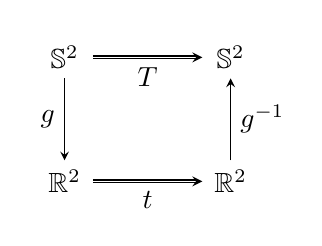
\begin{tikzpicture}
  \matrix (m) [matrix of math nodes,row sep=3em,column sep=4em,minimum width=2em]
  {
     \mathbb{S}^2 & \mathbb{S}^2 \\
     \mathbb{R}^2 & \mathbb{R}^2 \\};
  \path[-stealth]
    (m-1-1) edge node [left] {$g$} (m-2-1)
    (m-1-1) edge [double] node [below] {$T$} (m-1-2)
    (m-2-2) edge node [right] {$g^{-1}$} (m-1-2)
    (m-2-1) edge [double] node [below] {$t$} (m-2-2);
\end{tikzpicture}\end{center}\caption{Commutative diagram showing an naive approach to meshing on the sphere by converting the problem to the plane}\label{commutative_diagram}\end{figure}

A map $g: \mathbb{S}^2 \to \mathbb{R}^2$ must be choosen and an optimal transport map $t$ found. The boundary conditions for the problem of finding $t$ must be specified, and those boundary conditions would necessarily depend on $g$. For example in the case where the mapping $g$ is simply the lat-lon decomposition of $\mathbb{S}^2$, the boundary conditions for the mesh redistribution problem on the plane will then be periodic in the zonal direction. In the the meridional direction, Neumann boundary conditions would not be appropriate as the poles will not be free to move and they will be mapped back to their original location under $g^{-1}$. 

The Hairy Ball Theorem tells us that there must be at least one fixed point of the map $T: \mathbb{S}^2 \to \mathbb{S}^2$. The decomposition $T = g^{-1} \circ t \circ g$ would then be possible if $g$ maps the fixed points of $T$ to a Neumann boundary of $\mathbb{R}^2$. However the location of the fixed points of $T$ are not known \textit{a priori}, and hence choosing $g$ appropriately would form a significant problem by itself.



\bibliographystyle{unsrt}
\bibliography{/home/pbrowne/latex/bib/library,/home/pbrowne/Documents/Mendeley/library,/home/pbrowne/Dropbox/latex/bibliography}
\end{document}
